\documentclass[13pt]{scrreprt}
\usepackage[utf8]{inputenc} % use utf8 file encoding for TeX sources
\usepackage[T1]{fontenc}    % avoid garbled Unicode text in pdf
\usepackage[german]{babel}  % german hyphenation, quotes, etc
\usepackage{hyperref}       % detailed hyperlink/pdf configuration
\usepackage{graphicx}       % provides com\dfrac{m}{Nenner}ands for including figures
\usepackage{csquotes}       % provides \enquote{} macro for "quotes"
\usepackage[nonumberlist]{glossaries}     % provides glossary commands
\usepackage{enumitem}
\usepackage[center]{caption}
\usepackage[export]{adjustbox}
\newcounter{tempcounter1}
\newcounter{tempcounter2}
\newcounter{tempcounter3}
\newcounter{tempcounter4}
\newcounter{tempcounter5}
\newcounter{tempcounter6}
\newcounter{tempcounter7}
\newcounter{tempcounter8}
\newcounter{tempcounter9}

\makenoidxglossaries


\title{
	
\includegraphics[scale=0.5,center]{OfficialLogo.png}
	\\
Implementierungsbericht
}
\author{\\ \\ \\ \\ Marijan Petričević, Christoph Hartmann, Clara Walendy,\\
	 Jakob Dräger, Julius Meißner}

\begin{document}
\maketitle

% Platzierung des Inhaltsverzeichnisses
\tableofcontents

\chapter{Einleitung}
Dieses Dokument beschreibt die Implementierungsphase der Software Graphitty.
Es zeigt die Änderungen, die während der Entwicklung gemacht wurden und dokumentiert die implementierten Muss- und Wunschkriterien.\\
Die Anwendung ist im Rahmen des Pflichtmoduls Praxis der Softwareentwicklung des Bachelor-Studiengangs Informatik am Karlsruher Institut für Technologie entstanden. Das Projekt wurde am Lehrstuhl für Systeme der Informationsverwaltung angeboten.\\ Graphitty soll die Forschung in der Graphentheorie erleichtern. Die Software soll einen Forscher dabei unterstützen Korrelationen zwischen Merkmalen von Graphen und der Totalfärbungsvermutung zu finden.\\
Das Dokument ist das Artefakt der Implementierungsphase und zeigt den Stand der Implementierung, die Probleme bei der Implementierung, die Unittests, sowie eine Anleitung für die Erweiterung der Software.

\chapter{Übersicht}
\section{Versionskontrolle und Hilfsmittel}
Das Projekt wird mithilfe von Git entwickelt. Das Visual Studio Plug-In CodeMaid sorgt für standardisierten und aufgeräumten Code.
Es wird ein privates Repository verwendet, um die Entwicklung privat zu halten.\\
Da es auf Grund unterschiedlicher Module nicht zu Konflikten zwischen Entwicklern kommt, wurde sich gegen Continueous Integration entschieden.\\
Tests werden über die Komponententests in C\# ausgeführt.


\chapter{Änderungen am Entwurf}
Im Folgenden werden die Änderungen zum Entwurfsdokument genannt und näher beschrieben.
Die Aufteilung erfolgt in die bekannten Module und Klassen.

\section{Modul Data Access Layer}
	\subsection{Klasse UnitOfWork}
	Die \textit{UnitofWork} wurde um die Methoden \textit{Connect(string database)} und \textit{Delete(string Database)} erweitert. Diese ermöglichen einem Nutzer sich mit einer Datenbank zu verbinden (sollte die Datenbank mit dem Namen nicht existieren, so wird diese vorher erstellt) oder eine Datenbank zu löschen.
	\\
	Zudem wurden auch zwei neue Properties hinzugefügt. Eine bietet eine Liste von allen verfügbaren Datenbanken des aktuellen Servers an. Diese lautet: \textit{List<string> AvailableDatabases}. Die Zweite Property bietet einen standard Datenbanknamensprefix an, der verwendet wird wenn eine neue Datenbank erstellt wird. Die Property lautet: \textit{static string DatabasePrefix}.

\section{Modul Graphen}
	\subsection{Klasse GraphEntity}
	Es wurden einige Properties der \textit{GraphEntity} Klasse geändert:
	\newline
	Die Property \textit{IsTotallyColorable} wurde umbennant in \textit{IsTCCFulfilled}.
	\newline
	Es wurde eine neue Property \textit{string BFSBitVektor} hinzugefügt die den BFS Code als Bitvector darstellt.
	\newline
	Die Property \textit{int BFSDensity} wurde entfernt.
	
	\newpage
	\subsection{Klasse Graph}
	Der Klasse \textit{Graph} wurde ein weiterer Konstruktor hinzugefügt, welcher einen Graphen aus einem BFSCode instanziiert. 
	Die Methode \textit{CompareProfile()} gibt nun eine boolsche Variable zurück, um einen klareren Vergleich zu bieten.
		
	\subsection{Klasse Vertex}
	Die Klasse \textit{Vertex} hatte im Entwurf das Attribut \textit{VColor : Color}. Der Datentyp wurde zu \textit{Brush} geändert.
	Dies bedeutet, das eine Farbe nicht mittels RGB-Werten angegeben wird, sondern über den Brushes-Enumerator.
	Statt der \textit{Compare}-Methoden implementiert die Klasse nun das \textit{IEquatable} Interface, wobei die \textit{Compare}-Methode durch eine \textit{Equals}-Methode ersetzt wurde.
	Außerdem wurden der Klasse \textit{Vertex} die Public Properties \textit{Degree} und \textit{BFSID} vom Typ Integer hinzugefügt, welche für die Anwendung der Algorithmen benötigt werden.
	
	\subsection{Klasse Edge}
	Die Klasse \textit{Edge} hatte im Entwurf das Attribut \textit{EColor : Color}. Der Datentyp wurde zu \textit{Brush} geändert.
	Dies bedeutet, das eine Farbe nicht mittels RGB-Werten angegeben wird, sondern über den Brushes-Enumerator.
	Statt der \textit{Compare}-Methoden implementiert die Klasse nun das \textit{IEquatable} Interface, wobei die \textit{Compare}-Methode durch eine \textit{Equals}-Methode ersetzt wurde.
	Aufgrund der neuen Public Property \textit{Degree} der Klasse \textit{Vertex} wurde die Methode \textit{IncrementDegrees()} hinzugefügt, welche den Knotengrad beider Knoten in der Kante um 1 erhöht.
	
	\newpage
	\subsection{Klasse BFSCode}
	Es wurde die Klasse BFSCode zum Modul Graph hinzugefügt. Sie implementiert das \textit{IComparable} Interface um die Arbeit mit Listen zu erleichtern. Diese Entwurfsänderung erfolgte aufgrund stark verteilter BFSCode-Funktionalitäten, welche das Verständnis und die Übersichtlichkeit verschlechterten. Diese Klasse dient als Datenstruktur um mit dem BFSCode zu arbeiten.
	Sie bietet folgende Konstruktoren und Methoden:
	
	\begin{flushleft}
    \underline{\textbf{Konstruktoren:}}
    \newline
    \textit{public BFSCode(List<int[]> bfsCode): } Erzeugt ein BFSCode-Objekt mit Hilfe einer Liste von Kanten.
	\newline
	\textit{public BFSCode(String bfs): } Erzeugt ein BFSCode-Objekt mit Hilfe des BFSCode-Strings oder eines BitVector-Strings.
	\newline
	\underline{\textbf{Methoden:}}
	\newline
	\textit{public int CompareTo(BFSCode code): } Vergleicht den aktuellen BFSCode mit dem Übergebenen. Ist der übergebene nach BFS dichter wird 1 zurückgegeben. Bei Gleichheit 0. Ist der übergebene BFSCode weniger dicht, wird -1 zurückgegeben.
	\newline
	\textit{public String BFSToString(): } Gibt den BFSCode als String aus.
	\newline
	\textit{public String GetBitVector(): } Gibt den BFSCode als Bitvector-String zurück.
	\end{flushleft}
	\subsection{GraphsView}
	In der Klasse \textit{GraphsView} wurde ein Button zum Löschen von einzelnen Graphen hinzugefügt.
	
	\newpage
\section{Modul Algorithmen}
In sämtlichen Klassen wurden die Attribute entfernt, da diese überflüssig sind. Wegen dieser Änderung wurden Parameter und Rückgabetypen zu den Methoden hinzugefügt .Diese Änderungen werden nicht in jeder der folgenden Klasse genannt.

\subsection{AlgorithmRunner}
Der Klasse \textit{AlgorithmRunner} wurden Instanzen der Algorithmen und Compare Klassen in die Eigenschaften gegeben. Dies ist nötig um die \textit{Run}-Methoden der unterschiedlichen Algorithmen auszuführen. 

\subsection{Klasse Algorithmen}
Die Methode \textit{putGraphInProperties} wurde entfernt, da der Graph den Methoden übergeben wird.

\subsection{Klasse BreadthFirstSearch}
In der Klasse \textit{BreadthFirstSearch} wurde die Methode \textit{sortLexicographically} entfernt, da die Sortierung einer Liste von BFS-Codes mit der BFSCodes Klasse gemacht wird.
Es wurde auch \textit{findMinimalBFSCode} entfernt, da der minimale BFS-Code in der Methode \textit{breadthFirstSearch} gefunden wird.

\subsection{Klasse Comparison}
Die Klasse \textit{Comparison} hat im Entwurf von Algorithms geerbt. Dies ist nicht mehr der Fall, da zwei Graphen in den Compare Klassen bearbeitet werden, die in der \textit{Run}- Methode übergeben werden. 
\textit{Run(Graph graph)} wurde zu \textit{Run(Graph graph, GraphEntity dbGraph)} geändert, damit zwei Graphen übergeben werden können. 
Die Methode \textit{compare} wurde ebenfalls entfernt, da die Vergleiche direkt in der \textit{Run}-Methode ausgeführt werden.

\newpage
\section{Modul Filter}
	\subsection{IFilter und  Filterhierarchie}
	Um eine einfache Erweiterbarkeit der Filter zu gewährleisten, wurden Zwischenschritte in der Vererbungshierarchie eingeführt:\\
	
	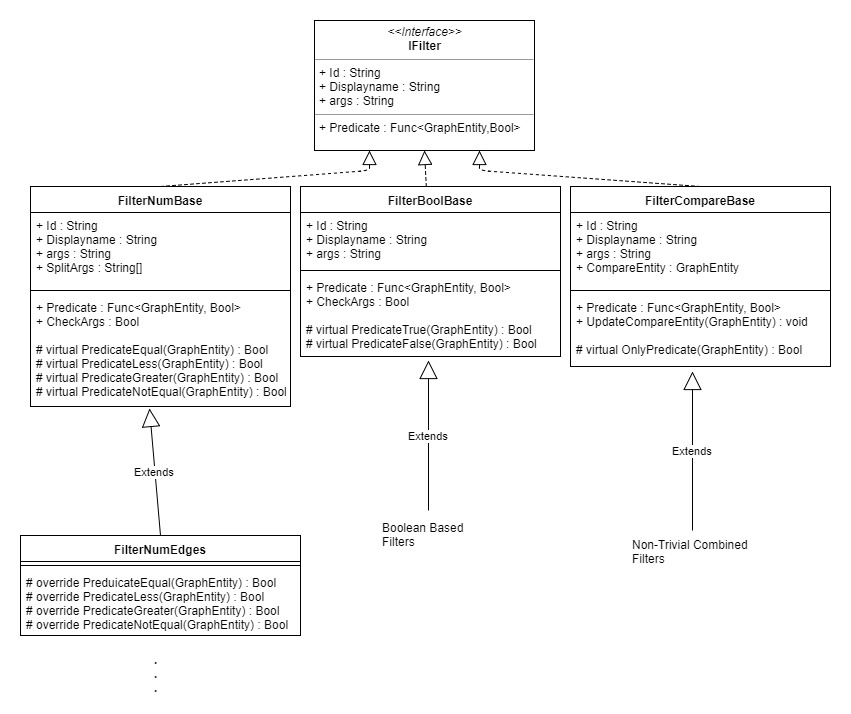
\includegraphics[scale=0.5,center]{FiltersNew.JPG}\\
	
	Diese \textit{Filter}<Typ>\textit{Base}-Klassen enthalten die gesamte Logik zur Filtererstellung. Dies ermöglicht dem Benutzer bei der Erweiterung nur das eigentliche Prädikat, die ID und den Filternamen anpassen zu müssen.
	
	\subsection{FiltersViewModel}
	Um die neuen Arten von Filtern benutzen zu können, musste das \textit{FiltersViewModel} (=\textit{FVM}) leicht verändert werden.
	Das \textit{FVM} abonniert das \textit{SelectionChangedEvent}, um eine Referenz auf den aktuell ausgewählten Graphen zu erhalten. Dies ist erforderlich für die vergleichenden Filter.
	\\
	Zusätzlich wurde die interne Struktur der Filterlisten verändert, damit die richtigen Informationen in die richtigen Filter eingefügt werden kann. Dies ist auch für die \textit{FiltersView} wichtig, damit die richtigen Parameter für jeden Filtertyp angezeigt werden.
	\\
	Das \textit{struct serializedFilter} wird benötigt, um die Daten als \textit{List<string,string>} zu speichern. Eine derartige Liste ist in C-Sharp ohne struct oder zusätzliche Klasse nicht möglich.
	\\
	Das automatische Updaten der gefilterten Liste wurde nicht umgesetzt.
	Stattdessen wurde ein Apply-Filter Button eingeführt, sodass sich die Auswahl nicht bei jeder Filteroperation ändert.
	
	\subsection{FilterItemViewModel}
	Diese neue Klasse trennt die Filter von der Benutzeroberfläche.
	
	\subsection{FiltersView}
	Die Filter werden nun anstatt in Kategorien, basierend auf den Merkmalen, in Kategorien, basierend auf dem Filtertyp sortiert.
	Diese Änderung macht das Erweitern einfacher, da die Darstellungslogik für einzelne Filter nun abhängig vom Typ des Filters ist (Siehe \textit{IFilter} und Filterhierarchie).

\section{Modul Graph Visualizer}
	\subsection{Klasse GraphToGUIConverter}
	Die Klasse hat zwei zusätzliche Methoden zur Zusammenhangsüberprüfung erhalten.
	Diese werden benötigt, um zu prüfen, ob ein Graph nach dem Bearbeiten gespeichert werden darf.
	Da ein Graph nur genau dann gespeichert werden darf, wenn er zusammenhängend ist, ist diese Überprüfung mittels DFS bereits in der Konvertierung von \textit{GUIGraph} zu \textit{Graph} eingebaut.
	Dies stellt sicher, das keine unzusammenhängenden Graphen in die Datenbank gelangen.
	
	\subsection{Klasse GraphVisualizerViewModel}
	Es wurde der \textit{ICommand SaveCommand} hinzugefügt, um das Speichern dem User zur Verfügung zu stellen, statt wie geplant automatisiert nach jeder Änderung.
	Dies ist durch die geforderte Zusammenhangseigenschaft auch nicht möglich.\\
	Da eine Färbung nicht in der Datenbank gespeichert wird, muss eine Neuberechnung der Färbung angestoßen werden.
	Zudem hat das \textit{GraphVisualizerViewModel} Zugriff auf die \textit{UnitOfWork} und den \textit{AlgorithmRunner}, um bearbeitete Graphen neu zu berechnen und schreibt diese anschließend in die Datenbank zurück.
	
	\subsection{Klasse GraphVisualizerView}
	Die Bedienung wurde auf Tool-Buttons umgestellt, um die Bedienung intuitiver und einheitlicher zu gestalten. Diese Buttons wurden auf der rechten Seite in der Graphenanzeige untergebracht.
	
\section{Modul Graph Generator}
	\subsection{Klasse Generator}
	Der Generator hat ein öffentliches Attribut \textit{TryGenerateThreshold} erhalten, welches dazu dient, der Generierung eine Abbruchbedingung zur Verfügung zu stellen, falls für die gegebene Fabrik- und Parameterkombination bereits alle möglichen Graphen in der Datenbank vorliegen. Dieses Obergrenze kann vom Benutzer vor Start der Generierung gesetzt werden.
	
	\newpage
	\subsection{Klasse FixedNumVerticesFactory}
	Diese Klasse implementiert das Interface \textit{IVertexFactory}  und generiert eine feste Anzahl an Knoten, welche sie zurückgibt. Sie wurde der Anwendung hinzugefügt, um vor allem das Testen und später das Demonstrieren der Datenbank zu vereinfachen. Die in der Implementierung als einzige Knoten-Factory vorgesehene \textit{MaxVerticesFactory} verteilt bei der Generierung die Graphen über viele Datenbanken, da sie mit einer randomisierten Knotenanzahl arbeitet. Dies erschwert unter Umständen, gerade bei noch kleinen Graphenbeständen, was bei initialer Demonstration der Fall sein wird, eine anschauliche und umfangreiche Darstellung der Filter- und Korrelationsberechnungsfunktionen.
	

\chapter{Implementierte Musskriterien}
Die unten stehenden Musskriterien sind erfüllt, wenn das Schlüsselwort \\ "DONE" hinter ihnen steht.
Die Auflistung enthält alle im Pflichtenheft spezifizierten Musskriterien.
\section{Grundfunktionalität}
\begin{addmargin}[25pt]{0pt}
	\begin{enumerate} [label=FA\arabic*,start=100]
		\item \label{FA100}Die Anwendung wartet nach dem Starten auf Benutzereingaben. DONE
		\item \label{FA101}Die Datenbank wird beim ordnungsgemäßen Schließen der Anwendung gesichert. DONE
		\setcounter{tempcounter3}{\value{enumi}}
	\end{enumerate}
\end{addmargin}

\section{Datenbank}
\begin{addmargin}[25pt]{0pt}
	\begin{enumerate} [label=FA\arabic*,start=200]
		\item \label{FA200}Die generierten Graphen werden nach der Anwendung der Algorithmen mit ihren Merkmalen in einer Datenbank gespeichert. DONE
		\item \label{FA201}Es können Graphen samt den dazu gespeicherten Merkmalen gelöscht werden. DONE
		\item \label{FA202}In einem beliebig ausgewähltem Graphen können Kanten entfernt oder hinzugefügt werden. DONE
		\item \label{FA203}Für den in \ref{FA202} modifizierten Graphen können die Merkmal neu berechnet werden. DONE
		\item \label{FA204}Der in \ref{FA202} und \ref{FA203} beschriebene Graph kann anschließend wieder in die Datenbank eingepflegt werden. DONE
		\item \label{FA205}Die Datenbank muss vom Datenbankmanagementsystem MariaDB verwaltbar sein können. DONE
		\setcounter{tempcounter4}{\value{enumi}}
	\end{enumerate}
\end{addmargin}

\section{Graphengenerierung}
\begin{addmargin}[25pt]{0pt}
	\begin{enumerate} [label=FA\arabic*,start=300]
		\item \label{FA300}Die Graphen werden zufallsbasiert generiert. DONE
		\item Standardmäßig werden Graphen mit einer Anzahl von 20 Knoten generiert. DONE
		\item Vor der Generierung soll es möglich sein eine eigene Anzahl von Knoten festzulegen. DONE
		\setcounter{tempcounter5}{\value{enumi}}
	\end{enumerate}
\end{addmargin}

\section{Grafische Benutzeroberfläche}
\begin{addmargin}[25pt]{0pt}
	\begin{enumerate} [label=FA\arabic*,start=400]
		\item \label{FA400}Durch Anwendung von Filtern soll es möglich sein, Graphen die diesen Filterkriterien entsprechen übersichtlich darzustellen. Dabei kann über alle in \ref{FA6} und folgende angegebenen Merkmal gefiltert werden. DONE
		\item \label{FA401}Die in \ref{FA400} genannten Filter sollen kombinatorisch anwendbar sein. DONE
		\item Es sollen die n am stärksten korrellierenden Merkmale angezeigt werden. DONE
		\item Korrelationen zwischen den verschiedenen Merkmalen sollen verdeutlicht werden, sofern die Merkmale stark korrelieren. DONE
		\setcounter{tempcounter6}{\value{enumi}}
	\end{enumerate}
\end{addmargin}

\section{Darstellung der Graphen}
\begin{addmargin}[25pt]{0pt}
	\begin{enumerate} [label=FA\arabic*,start=500]
		\item \label{FA500}Der generierte Graph soll dargestellt werden, indem die Knoten und Kanten grafisch angezeigt werden. DONE
		\item Existiert eine gültige Färbung, so wird diese dargestellt. DONE
		\item Die berechneten Merkmale sollen angezeigt werden. DONE
		\setcounter{tempcounter7}{\value{enumi}}
	\end{enumerate}
\end{addmargin}

\section{Graphenanalyse}
\label{Graphenanalyse}
Nachdem ein Graph generiert wird, werden folgende Merkmale bestimmt, beziehungsweise berechnet. \\
\begin{addmargin}[25pt]{0pt}
	\begin{enumerate} [label=FA\arabic*,start=600]
		\label{FA6}
		\item Anzahl der Knoten $n$ DONE
		\item Anzahl der Kanten $m$ DONE
		\item Durchschnittlicher Knotengrad $d$ DONE
		\item Maximaler Knotengrad $\Delta$ DONE
		\item Größe der größten im Graph enthaltenen Clique DONE
		\item Anzahl der Cliquen der Größe $k$ für $3 \leq k \leq n$ DONE
		\item Dichte gemäß BFS-Code DONE
		\item Anzahl der Graphen im Datenbestand mit höherer BFS-Dichte, als der betrachtete Graph (ausgehend von gleicher Knotenanzahl). DONE
		\item Dichte gemäß Profil DONE
		\item Anzahl der Graphen im Datenbestand mit höherer Profil-Dichte, als der betrachtete Graph (ausgehend von gleicher Knotenanzahl). DONE
		\item Ist die Totalfärbungsvermutung erfüllt? DONE
		\item Totalchromatische Zahl $\chi$ DONE
		\item Aufwand, um eine gültige minimale Färbung zu berechnen in Millisekunden DONE
		\item Anzahl der Graphen in der Datenbank mit gleicher Knotenanzahl NICHT SINNVOLL
		\item Anzahl der Graphen im Datenbestand mit kleinerer oder gleicher totalchromatischer Zahl, als der betrachtete Graph (ausgehend von gleicher Knotenanzahl). DONE
		\setcounter{tempcounter8}{\value{enumi}}
	\end{enumerate}
\end{addmargin}

\chapter{Implementierte Kannkriterien}

\section{Graphengenerierung}
\begin{addmargin}[25pt]{0pt}
	\begin{enumerate}[label=FA\arabic*,start=303]
		\item Zu dem im Moment gewählten Graphen lässt sich der nächst dichtere Graph generieren. DONE
		\item Für jeden generierten Graphen kann zusätzlich der nächst dichtere Graph generiert werden. DONE
		\item Für einen Graphen lässt sich sukzessive der nächst dichtere Graph bestimmen. DONE
	\end{enumerate}
\end{addmargin}

\section{Grafische Benutzeroberfläche}
\begin{addmargin}[25pt]{0pt}
	\begin{enumerate} [label=FA\arabic*,start=404]
		\item Falls Graphen-Merkmale Extremwerte annehmen, sollen diese gesondert hervorgehoben werden.
		\item Nachdem alle Graphen generiert wurden, werden diejenigen mit den extremsten Werten in der Übersicht dargestellt.
		\item Filterkonfigurationen sollen gespeichert werden können. DONE
	\end{enumerate}
\end{addmargin}

\section{Darstellung der Graphen}
\begin{addmargin}[25pt]{0pt}
	\begin{enumerate} [label=FA\arabic*,start=503]
		\item \label{FA503}Es soll eine Zoom-Funktion geben, mit der Ausschnitte des Graphen betrachtet werden können. DONE
		\item \label{FA504}Bei einer Detaildarstellung soll es möglich sein, den Ausschnitt zu bewegen, um andere Teile des Graphen sichtbar zu machen. DONE
	\end{enumerate}
\end{addmargin}

\section{Graphenanalyse}
\begin{addmargin}[25pt]{0pt}
	\begin{enumerate} [label=FA\arabic*,start=615]
		\item Anzahl unterschiedlicher Totalfärbungen mit $\chi$ Farben
	\end{enumerate}
\end{addmargin}


\chapter{Probleme und Verzögerungen bei der Implementierung}

\section{Algorithmen}
\subsection{Codes und Darstellungen}
Da die Anwendung stark auf den BFS-Codes aufbaut, war es wichtig, sich auf eine korrekte und funktionale Darstellung der BFS-Codes zu einigen.
Hier gab es Probleme mit ID's > 9 und dem Parsen von BFS Codes.
\subsection{NP-Schwere Algorithmen}
Fast alle der verwendeten Algorithmen sind NP-Schwer und haben damit eine exponentielle Laufzeit.
Dies brachte einige Probleme mit dem Entwurf der Algorithmen, da Laufzeiten in der Größenordnung von Tagen oder Wochen unerwünscht sind.
\subsection{Algorithmen Entwurf}
Viele der Algorithmen mussten für das Programm entweder komplett neu entworfen oder stark verändert werden. Dies war vor allem zeitintensiv und hat die Entwicklung der Software verlangsamt.
\subsection{Modul Abhängigkeiten}
In der Software bauen die Module aufeinander auf, ohne direkt miteinander verbunden zu sein. Dies bedeutet, dass das Testen der abhängigen Komponenten sehr schwer ist.
\subsection{Filter}
Die Filter waren in ihrer ursprünglichen Art nicht einfach erweiterbar.

\chapter{Unittests}
Die Unittests sind im Testprojekt \textit{GraphittyTest}. Alle Unittests basieren auf der TestClass von C\#
\section{Graph}
\subsection{Test: GraphFromBFSConstructor}
Erstellt aus einem gegebenen \textit{BFSCode}-String ein \textit{Graph}-Objekt und prüft ob alle Elemente des \textit{BFSCode}-Strings zum \textit{Graphen} richtig hinzugefügt wurden.

\subsection{Test: CompareBFS}
Erstellt zwei \textit{Graphen} mit gegebenen \textit{BFSCode}-String und prüft ob die Vergleiche des \textit{BFSCodes} das richtige Ergebnis liefern.

\subsection{Test: CompareProfil}
Erstellt zwei \textit{Graphen} mit gegebenen \textit{Profil}-String und prüft ob die Vergleiche des \textit{Profils} das richtige Ergebnis liefern.

\subsection{Test: CompareGraphs}
Erstellt zwei \textit{Graphen} mit gegebenen \textit{BFSCode}-String und prüft ob die Vergleiche der \textit{Graphen} das richtige Ergebnis liefern.

\subsection{Test: ContainsEdge}
Erstellt einen Graphen mit gegebener \textit{Vertex}- und \textit{Edge}-Liste und prüft ob die ContainsEdge-Methode die richtigen Ergebnisse zurückliefert.

\subsection{Test: ContainsVertex}
Erstellt einen Graphen mit gegebener \textit{Vertex}- und \textit{Edge}-Liste und prüft ob die ContainsVertex-Methode die richtigen Ergebnisse zurückliefert.

\subsection{Test: FindEdges}
Erstellt einen Graphen mit gegebener \textit{Vertex}- und \textit{Edge}-Liste und prüft ob die FindEdges-Methode das richtige Ergebnis zurückliefert.

\subsection{Test: FindVertex}
Erstellt einen Graphen mit gegebener \textit{Vertex}- und \textit{Edge}-Liste und prüft ob die FindVertex-Methode die richtigen Ergebnisse zurückliefert.

\newpage
\section{Edge}

\subsection{Test: EdgeConstructor}
Erstellt eine \textit{Edge} mit  zwei gegebenen \textit{Vertices} und prüft ob alle \textit{Vertices} in der \textit{Edge} enthalten sind.

\subsection{Test: ContainsVertex}
Erstellt eine \textit{Edge} mit  zwei gegebenen \textit{Vertices} und prüft ob die ContainsVertex-Methode die richtigen Ergebnisse zurückliefert.

\subsection{Test: GetVertices}
Erstellt eine \textit{Edge} mit  zwei gegebenen \textit{Vertices} und prüft ob die GetVertices-Methode das richtige Ergebnisse zurückliefert.

\subsection{Test: IncrementDegree}
Erstellt eine \textit{Edge} mit  zwei gegebenen \textit{Vertices} und prüft ob die IncrementDegree-Methode den \textit{Vertex-Degree} richtig erhöht.

\subsection{Test: Equals}
Erstellt drei \textit{Edges} mit drei \textit{Vertices} wovon zwei die gleichen \textit{Vertices} verwenden und prüft ob die Equals-Methode die richtigen Ergebnisse zurückliefert.

\newpage
\section{Vertex}

\subsection{Test: VertexConstructor}
Erstellt einen \textit{Vertex} mit einer vorgegebenen ID und prüft ob die ID und der Degree richtig gesetzt sind.

\subsection{Test: Equals}
Erstellt zwei \textit{Vertices} mit vorgegebenen IDs und prüft ob die Equals-Methode die richtigen Ergebnisse zurückliefert.

\section{BFSCode}

\subsection{Test: BFSCodeConstructor}
Erstellt zwei \textit{BFSCode}-Objekte mit einem vorgegebenen \textit{BFSCode}-String und Bitvektor. Dabei wird geprüft ob der vorgegebene \textit{BFSCode}-String gleich dem \textit{BFSCode.BFSCodeToString} und der Bitvektor gleich \textit{BFSCode.GetBitVektor} ist.

\subsection{Test: BFSCodeCompareTo}
Erstellt zwei \textit{BFSCode}-Instanzen mit vorgebenen \textit{BFSCode}-Strings und überprüft ob die CompareTo-Methode die richtigen Ergebnisse zurückliefert.
\newpage
\section{Generator}

\section{Algorithms}

\subsection{Test: Totalcoloring}
Berechnet die Totalfärbung zu einem bekannten \textit{Graphen}. Prüft, ob die totalchromatische Zahl übereinstimmt.

\subsection{Test : BreadthFirstSearch}
Berechnet einen BFS-Code und ein Profil zu einem bekannten \textit{Graphen} und überprüft, ob diese stimmen.

\subsection{Test: VertexDegrees}
Berechnet den durchschnittlichen und maximalen Knotengrad eines \textit{Graphen} und überprüft, ob diese stimmen.

\subsection{Test: CliqueSearch}
Findet die größte Clique eines bekannten \textit{Graphen} und berechnet wie viele Cliquen der Graph hat, die eine kleinere Größe haben als die größte Clique. Prüft, ob die Ergebnisse mit dem Graphen übereinstimmen.

\subsection{Test: CompareBFS}
Berechnet den BFS-Code zu vier bekannten \textit{Graphen} und bestimmt die Anzahl an dichteren \textit{Graphen} nach BFS-Code Dichte für jeden dieser Graphen. Es wird überprüft, ob die richtigen Ergebnisse in den \textit{Graphen} gespeichert werden.

\subsection{Test: CompareProfile}
Berechnet das Profil zu vier bekannten \textit{Graphen} bestimmt die Anzahl an dichteren \textit{Graphen} nach Profil Dichte für jeden dieser Graphen. Es wird überprüft, ob die richtigen Ergebnisse in den \textit{Graphen} gespeichert werden. 

\subsection{Test: CompareTotalChromaticNumber}
Erstellt eine Totalfärbung für vier bekannte \textit{Graphen} und bestimmt die Anzahl an \textit{Graphen} mit kleinerer oder gleicher totalchromatischer Zahl für alle \textit{Graphen}. Es wird überprüft, ob die richtigen Ergebnisse in den \textit{Graphen} gespeichert werden.
\chapter{Erweiterbarkeit}

\section{Merkmale}
Um neue Merkmale hinzuzufügen, müssen die Module \textit{Graph}, \textit{Filter} und \textit{Algorithmen} geändert werden.
\subsection{Modul Graph}
Um den Graphen selbst und auch die Datenbank zu erweitern, muss zunächst die Klasse \textit{GraphEntity} erweitert werden. \\
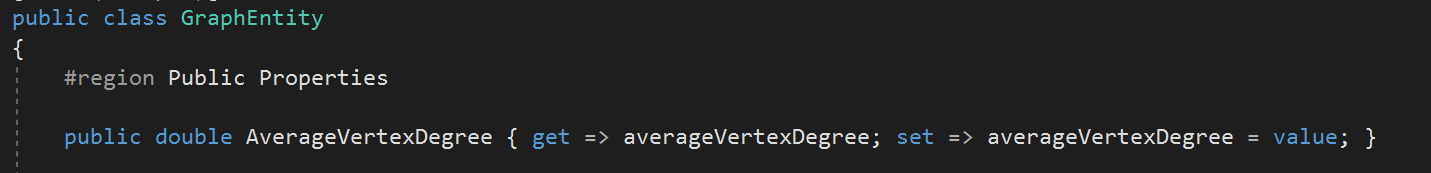
\includegraphics[scale=0.5,center]{db_ge.PNG}\\
Anschließend muss die Datenbank auf die neue Version migriert werden. Dies funktioniert folgendermaßen:\\\\
Schritt 1: Paketmanager öffnen\\
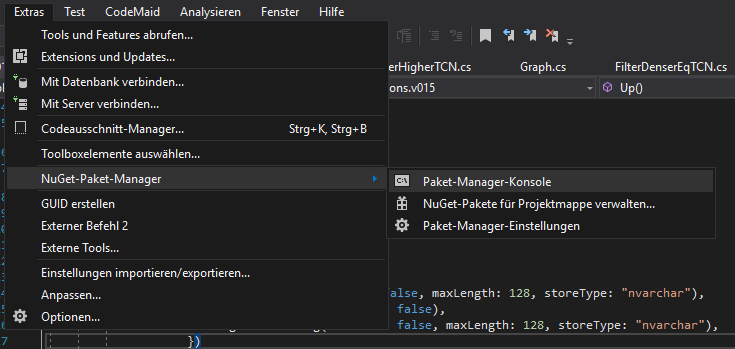
\includegraphics[scale=0.5,center]{db_pkgmng.PNG}\newpage
Schritt 2: Neue Migration erstellen mit dem Befehl:\textit{add-migration <Name> } ggfs. Option \textit{-force} hinzufügen.
\\
Vorher sollten Migrationen erlaubt werden, sollte dies nicht schon der Fall sein: \textit{enable-migrations}.
\\
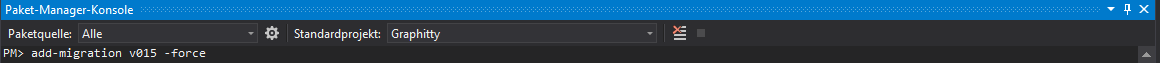
\includegraphics[scale=0.5,center]{db_addmig.PNG}\\\\
Schritt 3: Datenbank updaten mit dem Befehl \textit{update-database -verbose}. Eventuell muss die Datenbank vorher gelöscht werden.\\
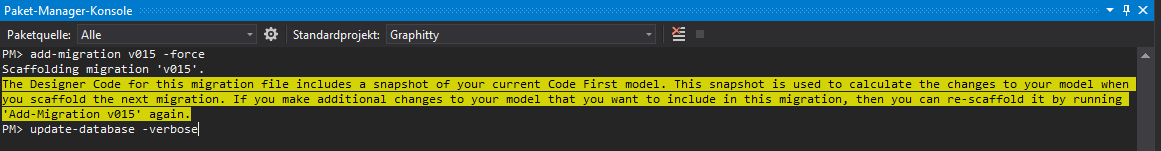
\includegraphics[scale=0.5,center]{db_updatedb.PNG}\\

\subsection{Modul Filter}
Damit die Datenbank nach dem neuen Merkmal gefiltert werden kann, muss ein neuer Filter erstellt werden. Hierzu werden die Klassen \textit{FilterNumBase}, \textit{FilterBoolBase} oder \textit{FilterCompareBase} vererbt, je nach gewünschtem Filtertyp.\\
Im neu erstellten Filter müssen nun die Variablen \textit{Id} und \textit{Displayname} im Konstruktor gesetzt werden.\\
Für die eigentliche Filterfunktionalität müssen die \textit{Predicates} überschrieben werden:
\newpage
FilterNumBase:\\
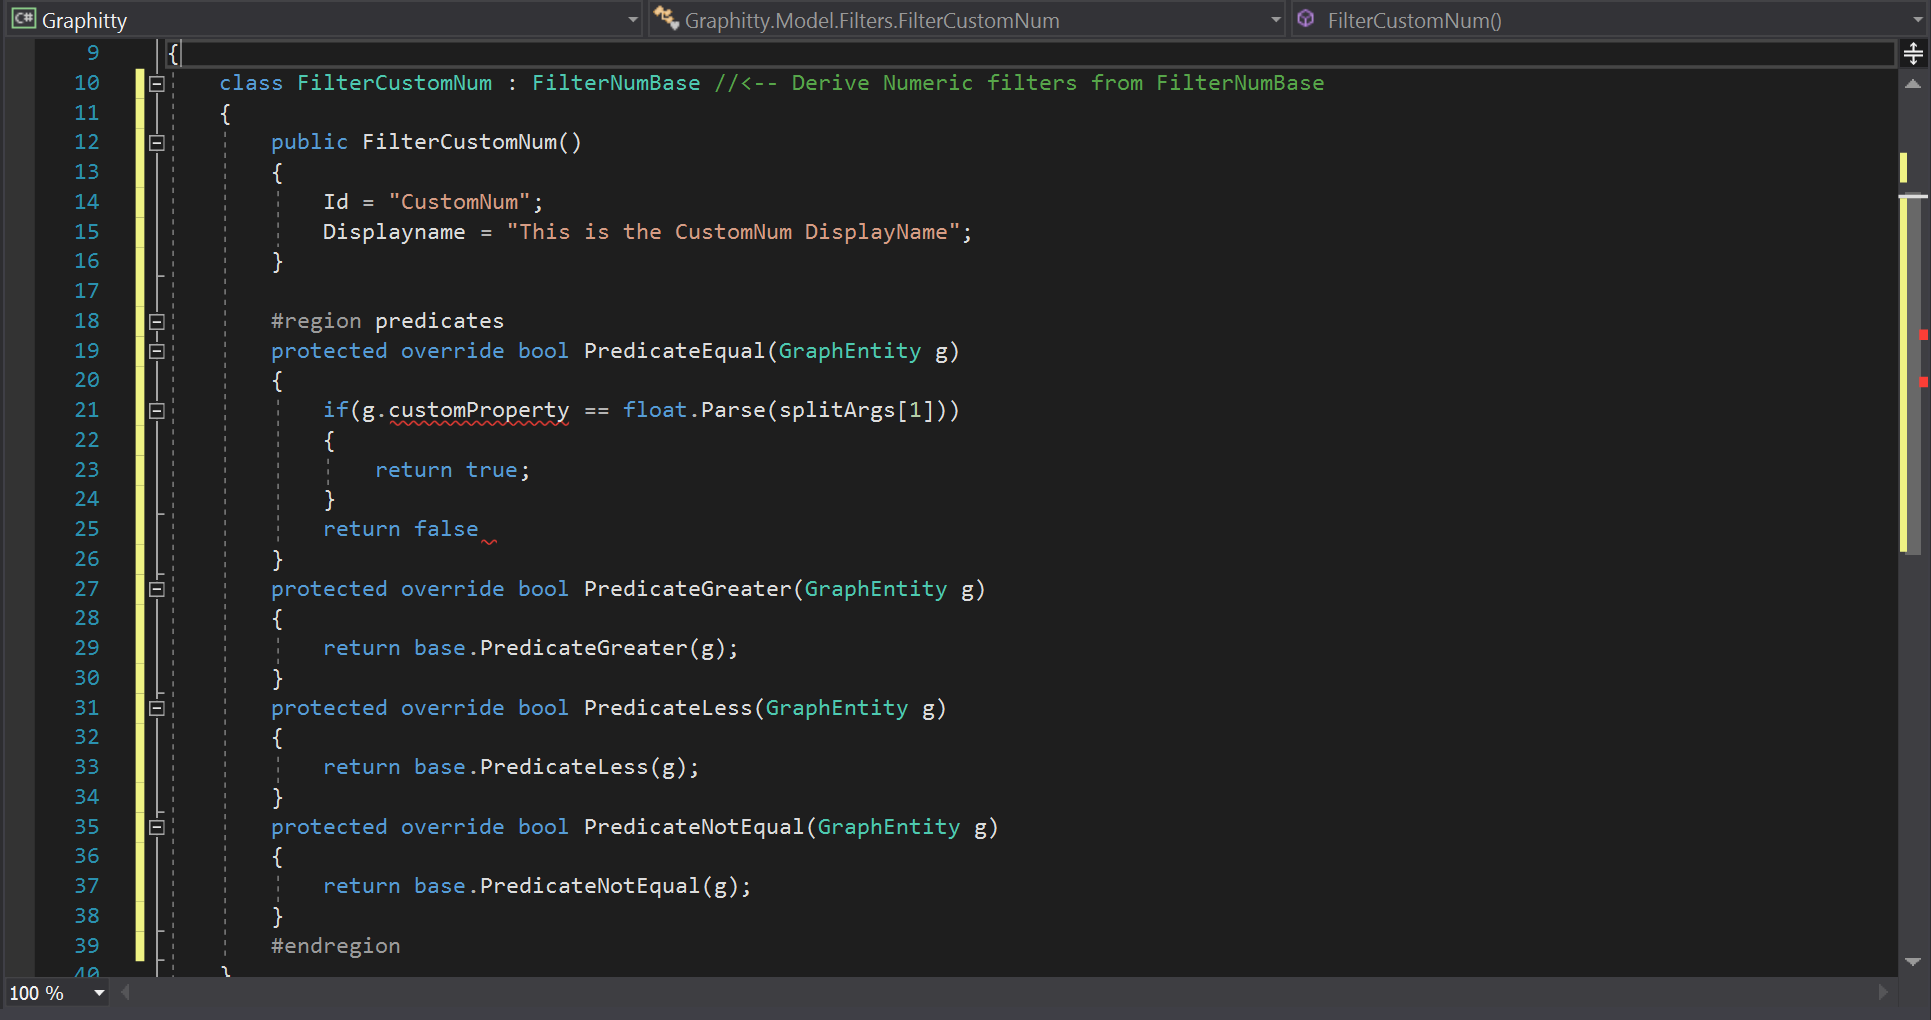
\includegraphics[scale=0.5,center]{FilterNumBase.PNG}
FilterBoolBase:\\
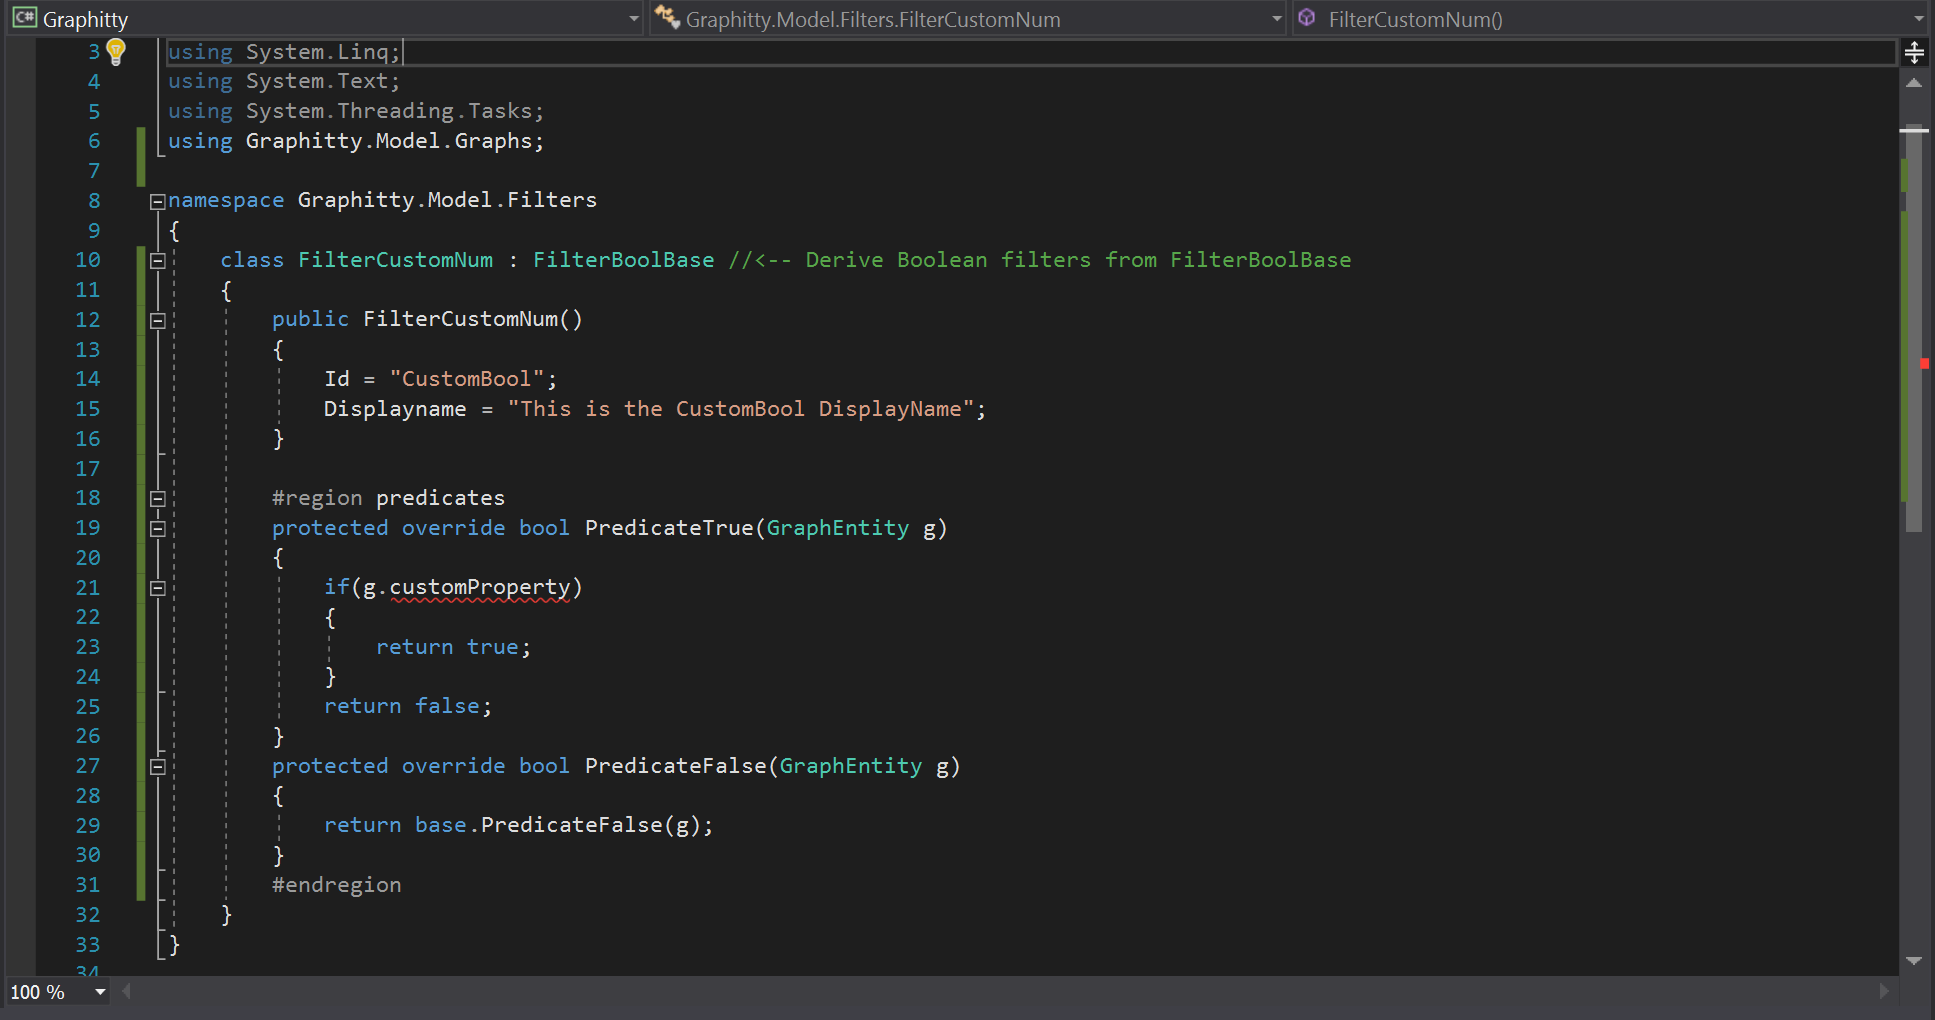
\includegraphics[scale=0.5,center]{FilterBoolBase.PNG}
\newpage
FilterCompareBase:\\
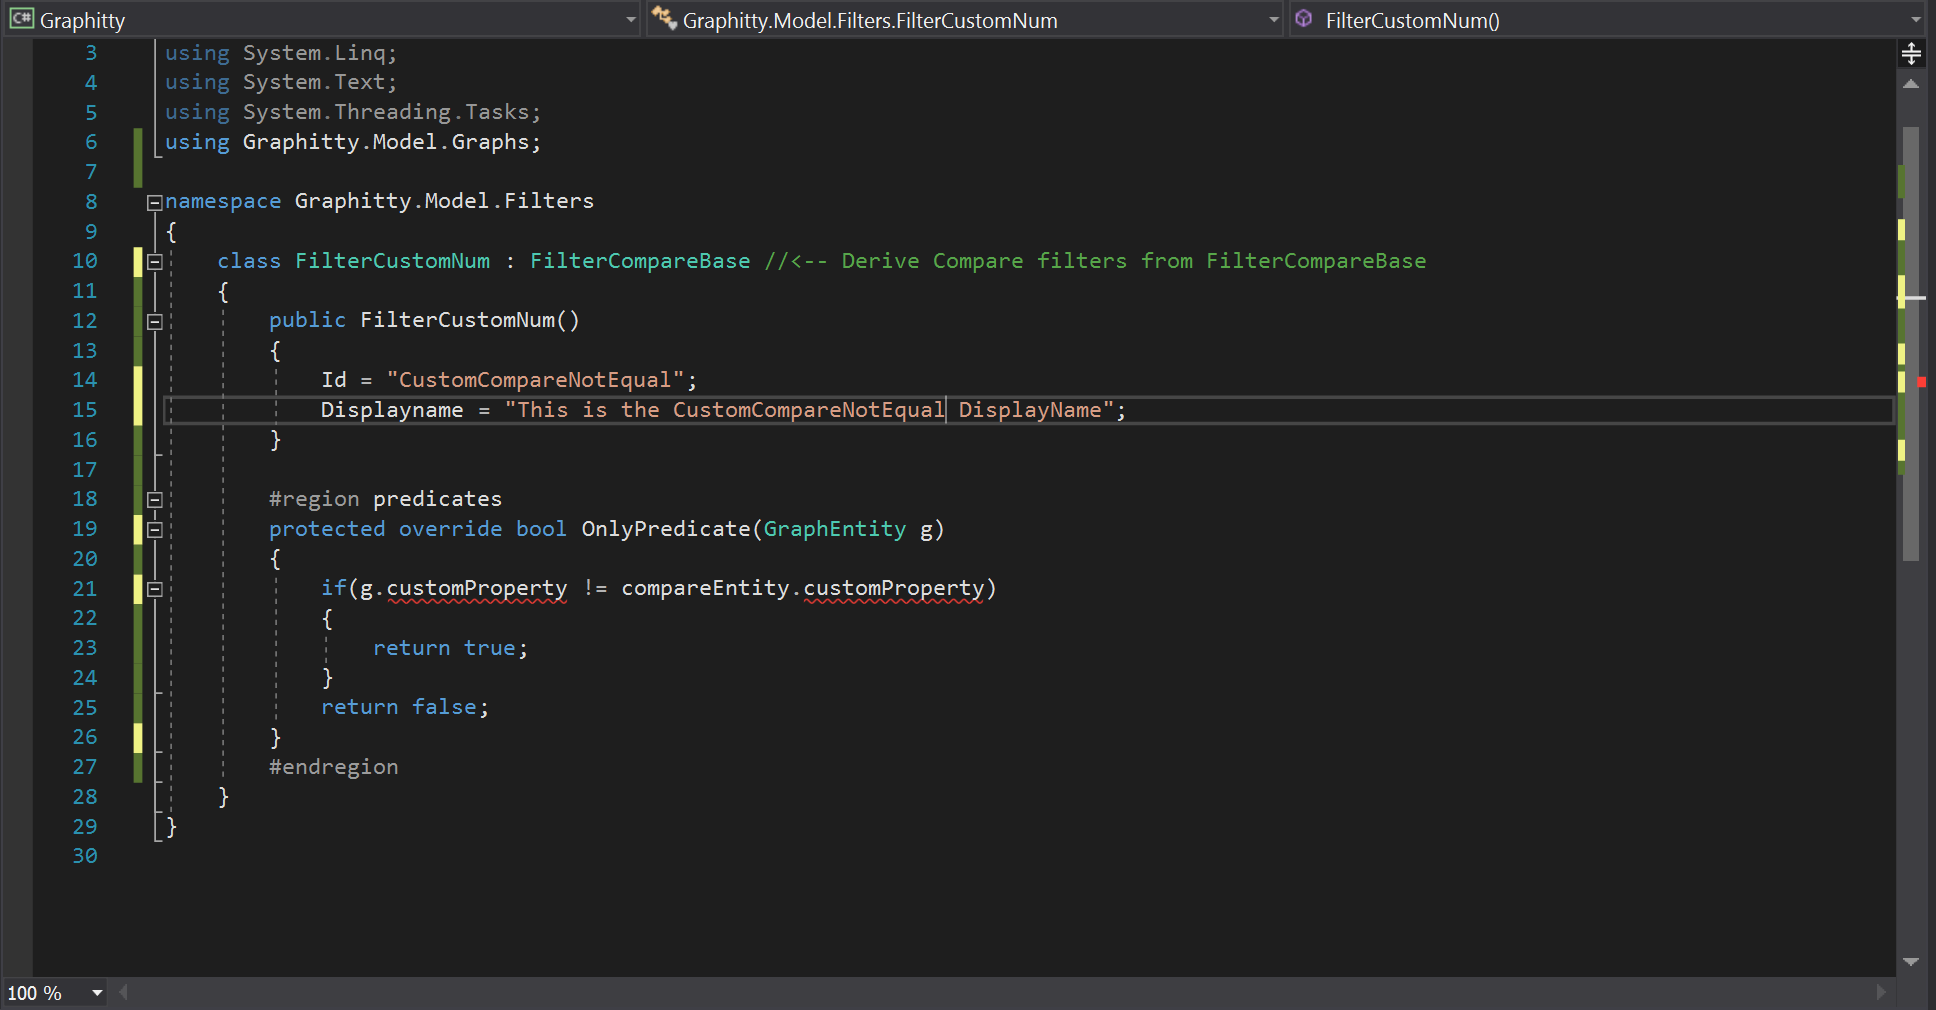
\includegraphics[scale=0.5,center]{FilterCompareBase.PNG}\\
Der letzte Schritt ist den Filter in das \textit{FiltersViewModel} einzufügen:\\
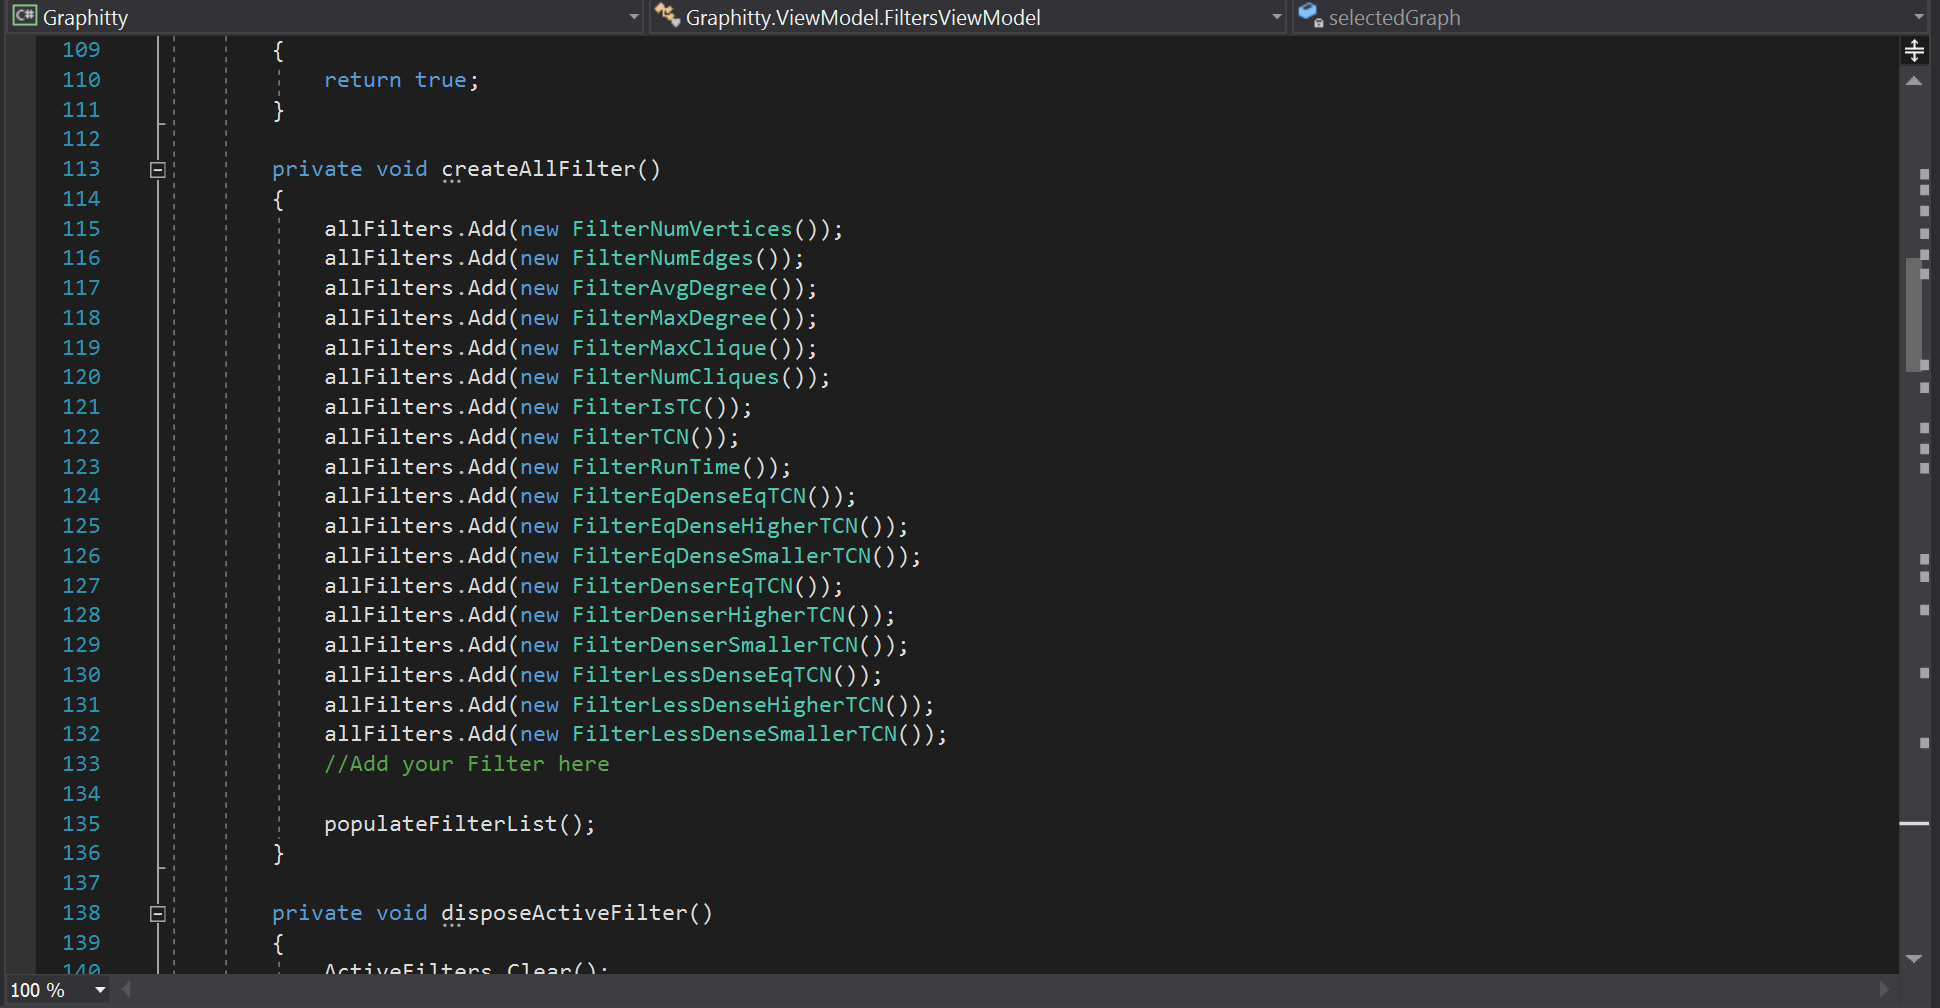
\includegraphics[scale=0.5,center]{FilterViewModel.PNG}

\newpage

\subsection{Modul Algorithmen}
Es muss ein neuer Algorithmus erstellt werden, der von der Klasse \textit{Algorithm} oder von der Klasse \textit{Comparison} erbt.\\
Wenn zwei Graphen verglichen werden, soll von \textit{Comparison} geerbt werden, in allen anderen Fällen wird von \textit{Algorithm} geerbt. In neuen Compare oder Algorithmen Klassen muss \textit{Graphitty.Model.Graphs} verwendet werden.
Die Algorithmen und die Vergleiche werden mit der \textit{Run}-Methode ausgeführt.
Alle errechneten Merkmale müssen in der \textit{GraphEntity} gespeichert werden.\\
In der Klasse \textit{AlgorithmRunner} muss eine Instanz der neuen Klasse hinzugefügt werden. Diese muss im Konstruktor initialisiert werden. Die \textit{Run}-Methode muss der \textit{RunAlgorithms}-Methode hinzugefügt werden.\\
\\

Algorithmen Klasse:\\
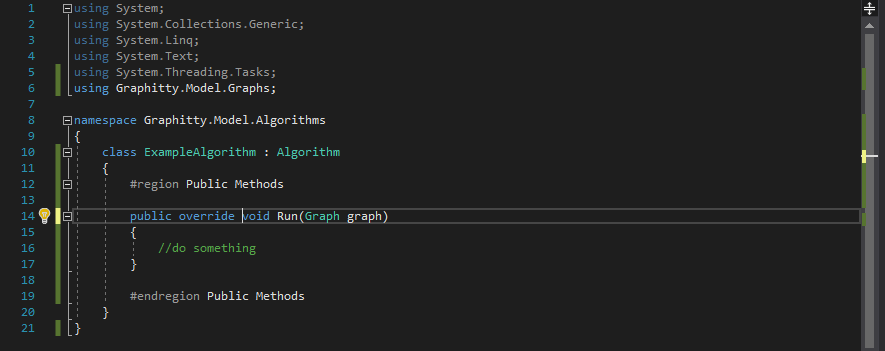
\includegraphics[scale=0.7,center]{algorithm.PNG}
\newpage
Comparison Klasse:\\
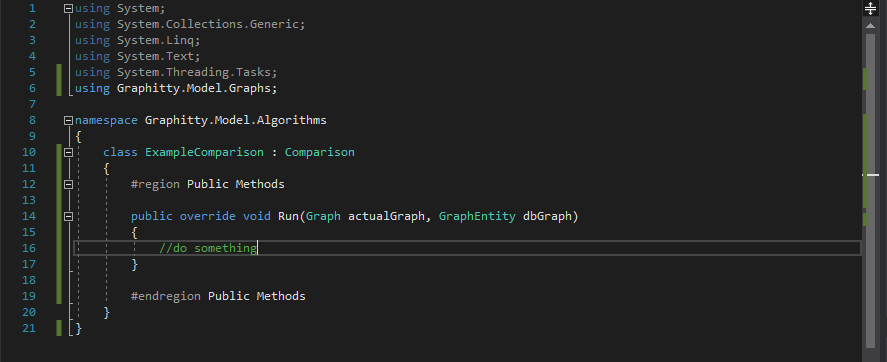
\includegraphics[scale=0.7,center]{comparison.PNG}
AlgorithmRunner Klasse:\\
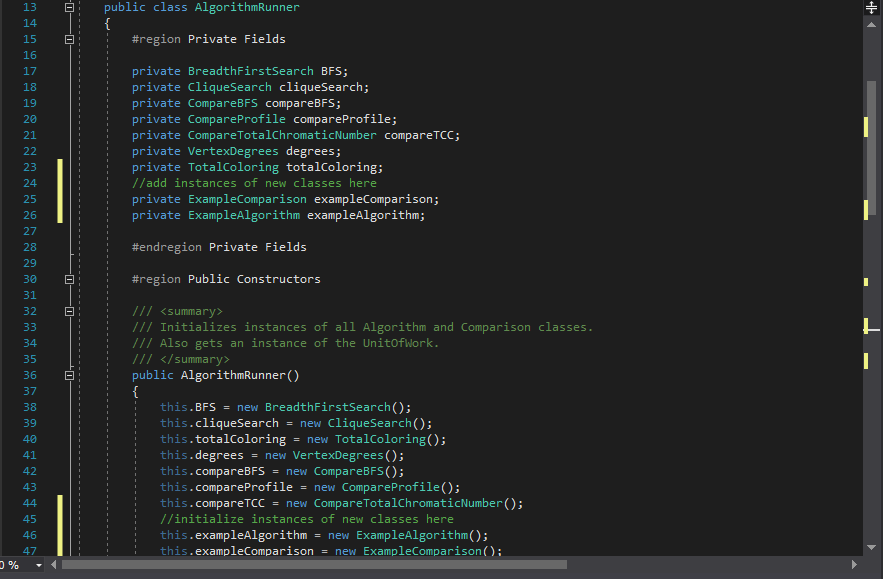
\includegraphics[scale=0.7,center]{algorithmrunner.PNG}
\newpage
RunAlgorithms Methode:\\
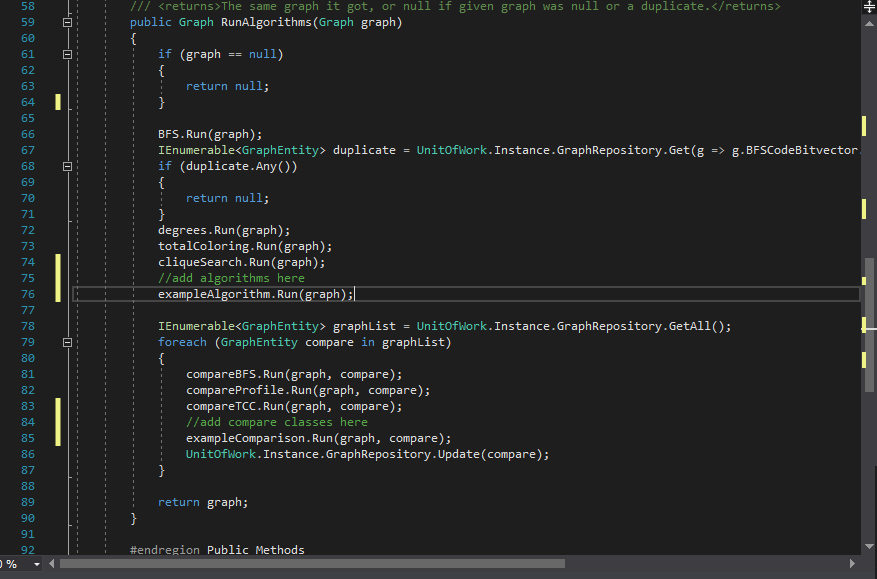
\includegraphics[scale=0.7,center]{runAlgorithms.PNG}
\newpage

\section{Graph Generator}
Die Generierung von neuen Graphen ist wie schon im Entwurf beschrieben durch die Implementierung der Interfaces \textit{IVertexFactory} und \textit{IEdgesFactory} erweiterbar. Die implementierenden Klassen, welche im Folgenden Fabriken genannt werden, m{\"u}ssen ihre ben{\"o}tigten Parameter als {\"o}ffentliche Attribute zur Verf{\"u}gung stellen, sodass das jeweilige ViewModel eine {\"A}nderung der Werte durch den Benutzer umsetzen kann. Um die angesprochene Kommunikation und die Anzeige aller zur Laufzeit verf{\"u}gbaren Fabriken zu realisieren, muss durch Implementierung der Interfaces \textit{IVertexFactoryViewModel} beziehungsweise \textit{IEdgesFactoryViewModel} ein ViewModel zur neuen Fabrik bereitgestellt werden. Die Viewmodels müssen einen Konstruktor ohne Argumente anbieten, welcher im \textit{GeneratorViewModle} an entsprechender Stelle (siehe Abbildung) aufgerufen werden muss. F{\"u}r jede Fabrik, welche spezifische Parameter verwendet, muss in \textit{FactoryViewTemplates} an entsprechender Stelle (siehe Abbildung) ein Data-Template erstellt werden, in welches der Benutzer die ben{\"o}tigten Parameter eintragen kann.

\newpage
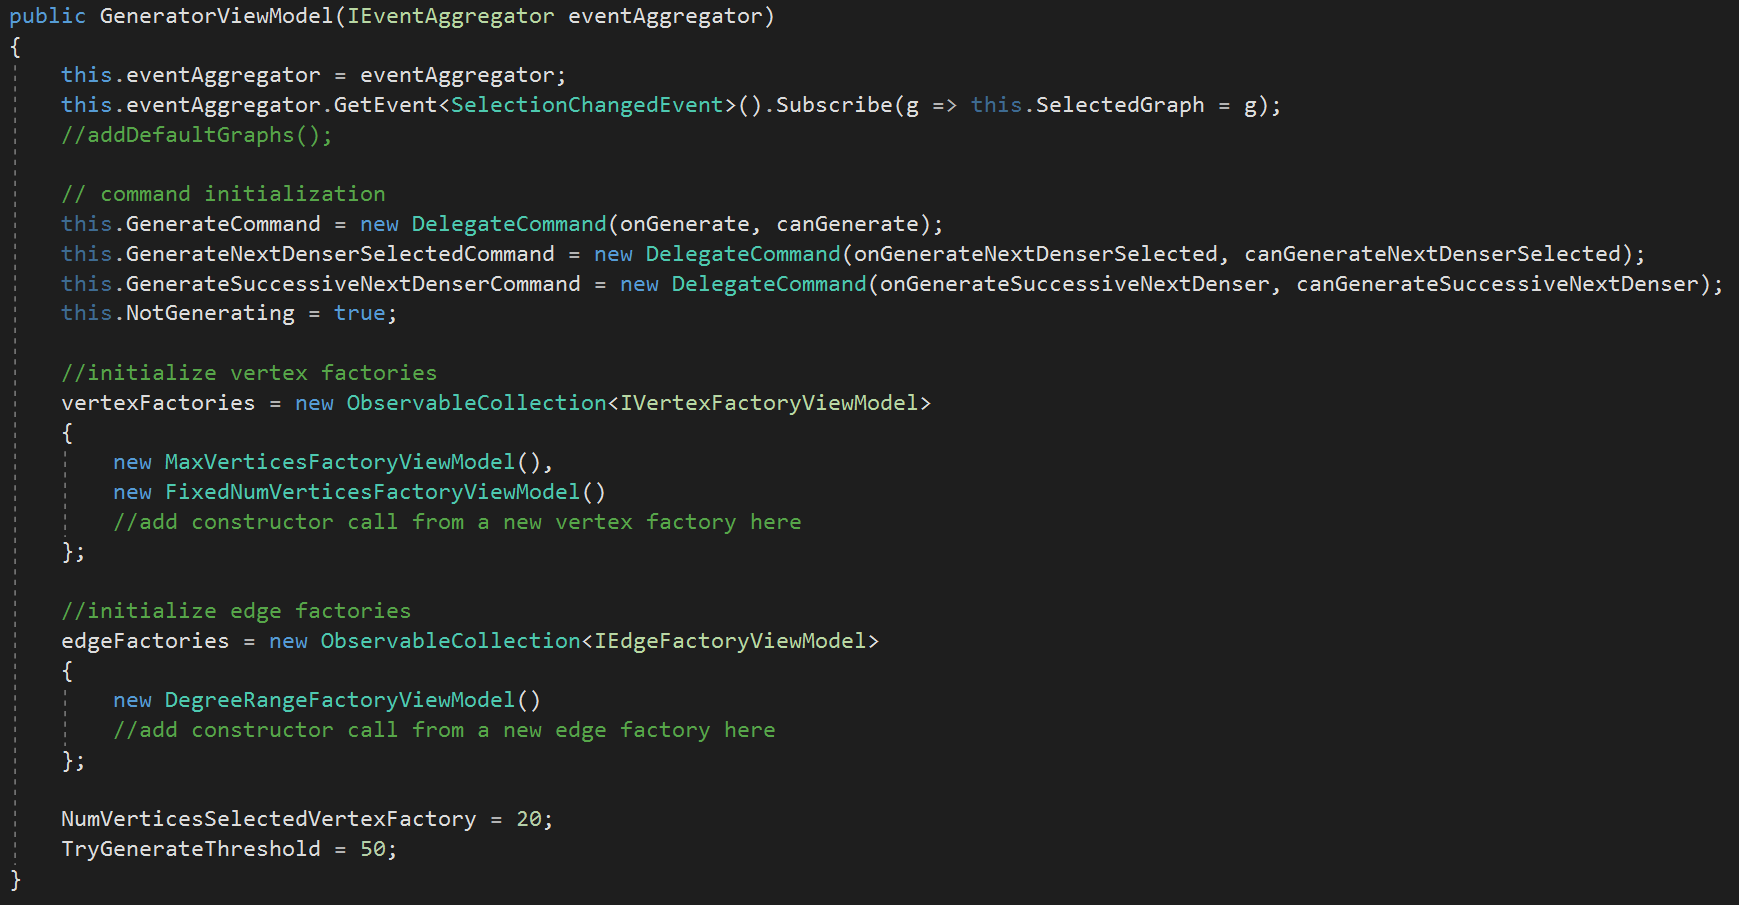
\includegraphics[scale=0.6,center]{GeneratorViewModelKonstruktor.PNG}
Abbildung \textit{GeneratorViewModle}
\\ \\

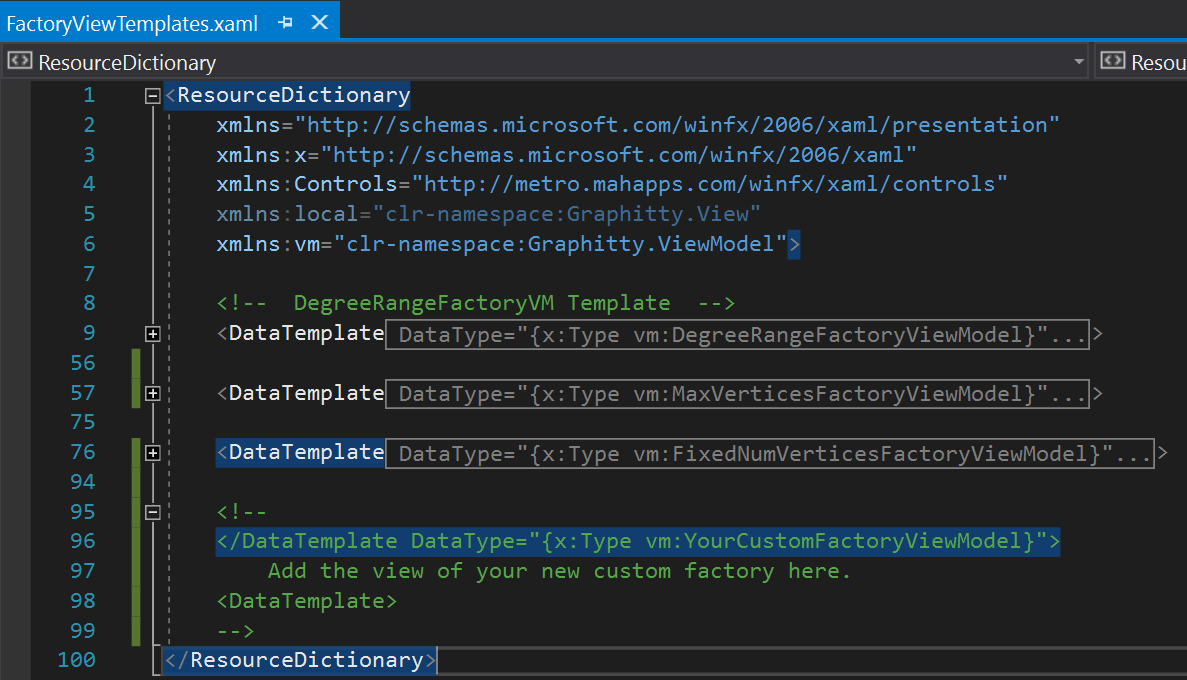
\includegraphics[scale=0.87,center]{FactoryViewDataTemplate.PNG}
Abbildung \textit{FactoryViewTemplates}

\glsaddall
\printnoidxglossaries

\end{document}
